\documentclass[answers]{exam}
\usepackage{texPreamble}
\usepackage{relsize}
\usepackage{tabularx}
\extraheadheight{0.25in}
\extrafootheight{1.0in}
\extrawidth{1in}
% ----------------------------------------------------------------
\firstpagefootrule
\runningfootrule
\begin{document}
%\relscale{1.4}
\section{5.1: Approximating Areas under Curves}
\begin{center}
  \begin{tikzpicture}
    \begin{groupplot}[
      group style={group size=2 by 1, horizontal sep=2in},
      width=0.35\linewidth,
      axis lines=center,
      axis line style={->},
      ticklabel style={font=\footnotesize,inner sep=0.5pt,fill=white,opacity=1.0, text opacity=1},
      xlabel=$x$, xlabel style={at={(ticklabel* cs:1)},anchor=north west},
      ylabel=$y$, ylabel style={at={(ticklabel* cs:1)},anchor=south west},
      every axis plot/.append style={line width=0.95pt, color=blue, samples=100}
      ]
      \nextgroupplot[
        xmin=-0.5, xmax=6.5,
        ymin=-0.5, ymax=2.5,
        ]
        \def\f(#1){1/8*(#1)^3-3/2*(#1)^2+23/4*(#1)-5};
        \draw[fill=blue!50, opacity=0.75] plot[smooth, samples=100, domain=2.5:5] (\x,{\f(\x)}) |- (2.5,0) -- cycle;
        \addplot[name path=f, -] expression[domain=0:6]{\f(\x)};
      \nextgroupplot[
        xmin=-0.25, xmax=1.15,
        xtick={0,1},
        ymin=-0.25, ymax=1.25,
        ]
        \def\f(#1){1-(#1)^2};
        \draw[fill=blue!50, opacity=0.75] plot[smooth, samples=100, domain=0:1] (\x,{\f(\x)}) |- (0,0) -- cycle;
        \addplot[name path=f, -] expression[domain=0:1]{\f(\x)} node[above right, pos=0.4, black, inner sep=0.5pt] {\normalsize $f(x)=1-x^2$};
    \end{groupplot}
  \end{tikzpicture}
\end{center}
Finding the area under the curve is simple in some cases:
  \begin{center}
    \begin{tikzpicture}
      \begin{groupplot}[
        group style={group size=2 by 1, horizontal sep=2in},
        axis lines=center,
        axis equal,
        width=0.35\linewidth,
        axis line style={->},
        ticklabel style={font=\footnotesize,inner sep=0.5pt,fill=white,opacity=1.0, text opacity=1},
        xlabel=$x$, xlabel style={at={(ticklabel* cs:1)},anchor=north west},
        ylabel=$y$, ylabel style={at={(ticklabel* cs:1)},anchor=south west},
        every axis plot/.append style={line width=0.95pt, color=blue, samples=100}
        ]
        \nextgroupplot[
          xmin=-2.5, xmax=2.5,
          ymin=-0.5, ymax=2.5,
          ]
          \def\f(#1){sqrt(4-(#1)^2)};
          \draw[fill=blue!50, opacity=0.75] plot[smooth, samples=100, domain=-2:2] (\x,{\f(\x)}) |- (2.5,0) -- cycle;
          \addplot[name path=f, -] expression[domain=-2:2, samples=751]{\f(\x)} node[above right, pos=0.52, black, inner sep=0.5pt] {\normalsize $f(x)=\sqrt{4-x^2}$};
        \nextgroupplot[
          xmin=-0.25, xmax=3.25,
          ymin=-0.25, ymax=3.25,
          ]
          \def\f(#1){-(#1)+3};
          \draw[fill=blue!50, opacity=0.75] plot[smooth, samples=100, domain=0:3] (\x,{\f(\x)}) -| (0,0) -- cycle;
          \addplot[name path=f, -] expression[domain=0:3]{\f(\x)} node[above right, pos=0.55, black, inner sep=0.5pt] {\normalsize $f(x)=-x+3$};
      \end{groupplot}
    \end{tikzpicture}
    \vspace*{\stretch{1}}
    
    \hspace*{\stretch{1}}
    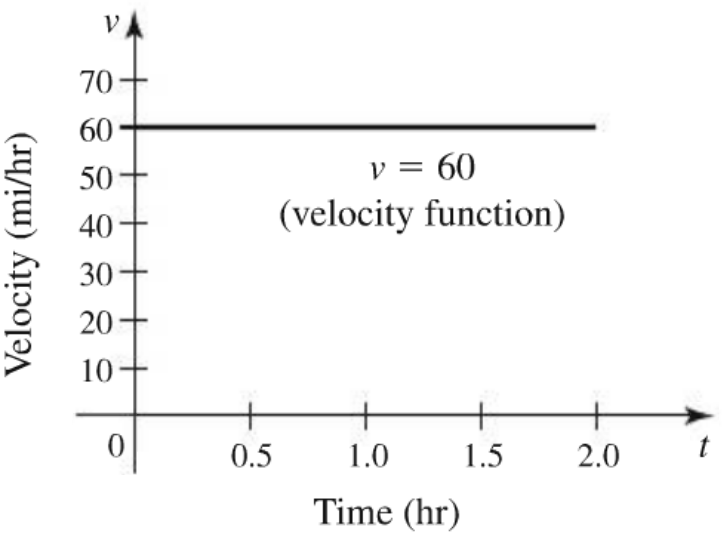
\includegraphics[width=0.35\linewidth]{images/briggs_05_01/velocityPlot_empty.png}
    \hspace*{\stretch{1}}
    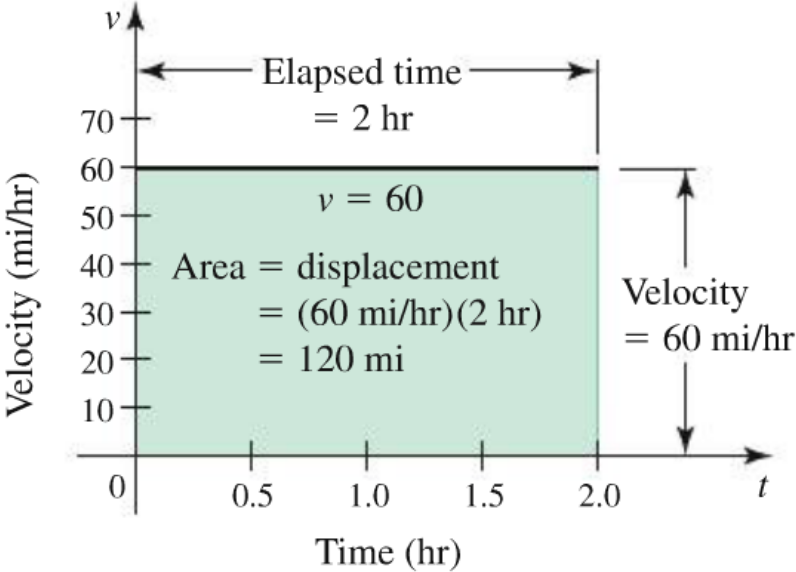
\includegraphics[width=0.35\linewidth]{images/briggs_05_01/velocityPlot_filled.png}
    \hspace*{\stretch{1}}
  \end{center}
\pagebreak

  For functions whose curves are irregular shapes, we can approximate the area using rectangles:
  \begin{center}
    \begin{tikzpicture}
      \begin{groupplot}[
        group style={group size=3 by 1, horizontal sep=0.25in},
        axis lines=center,
        xmin=-0.125, xmax=1.10,
        xtick={0,1},
        ymin=-0.125, ymax=1.25,
        width=0.375\linewidth,
        axis line style={->},
        ticklabel style={font=\footnotesize,inner sep=0.5pt,fill=white,opacity=1.0, text opacity=1},
        every axis plot/.append style={line width=0.75pt, color=blue, samples=100}
        ]
        \def\f(#1){1-(#1)^2};
        \def\a{0} \def\b{1}
        \def\n{4}            %% Number of rectangles
        %
        \FPsub\LEN\b\a       %% \LEN=\b-\a
        \FPdiv\del\LEN\n     %% \del=\LEN/\n
        \nextgroupplot
          \def\ALPHA{0.0}      %% left,center,right 0\leq \ALPHA\leq 1
          \FPmul\LR\del\ALPHA  %% \LR=\del*\ALPHA
          \pgfplotsinvokeforeach{\a,\a+\del,...,\b-\del}{
            \draw[left color=ClemsonPurple!75, right color=ClemsonPurple!40, line width=0.0pt] (axis cs: #1, 0) rectangle (#1+\del, {\f(\LR+#1)});}
          \addplot[name path=f, -] expression[domain=0:1]{\f(\x)};
        %
        %
        \nextgroupplot
        \def\ALPHA{0.5}      %% left,center,right 0\leq \ALPHA\leq 1
        \FPmul\LR\del\ALPHA  %% \LR=\del*\ALPHA
          \pgfplotsinvokeforeach{\a,\a+\del,...,\b-\del}{
            \draw[left color=ClemsonPurple!75, right color=ClemsonPurple!40, line width=0.0pt] (axis cs: #1, 0) rectangle (#1+\del, {\f(\LR+#1)});}
          \addplot[name path=f, -] expression[domain=0:1]{\f(\x)};
        %
        %
        \nextgroupplot
        \def\ALPHA{1.0}      %% left,center,right 0\leq \ALPHA\leq 1
        \FPmul\LR\del\ALPHA  %% \LR=\del*\ALPHA
          \pgfplotsinvokeforeach{\a,\a+\del,...,\b-\del}{
            \draw[left color=ClemsonPurple!75, right color=ClemsonPurple!40, line width=0.0pt] (axis cs: #1, 0) rectangle (#1+\del, {\f(\LR+#1)});}
          \addplot[name path=f, -] expression[domain=0:1]{\f(\x)};
      \end{groupplot}
    \end{tikzpicture}

    \begin{tabularx}{0.995\linewidth}{*{3}{Y}}
      Left rectangles&
      Midpoint rectangles&
      Right rectangles
    \end{tabularx}
  \end{center}
  \vspace*{\stretch{1}}
  
  These approximations are much more accurate when more rectangles are used:
  \begin{center}
    \begin{tikzpicture}
      \begin{groupplot}[
        group style={group size=3 by 1, horizontal sep=0.25in},
        axis lines=center,
        xmin=-0.125, xmax=1.15,
        ymin=-0.125, ymax=1.25,
        width=0.375\linewidth,
        axis line style={->},
        ticklabel style={font=\footnotesize,inner sep=0.5pt,fill=white,opacity=1.0, text opacity=1},
        every axis plot/.append style={line width=0.75pt, color=blue, samples=100}
        ]
        \def\f(#1){1-(#1)^2};
        \def\a{0} \def\b{1}
        \nextgroupplot[xtick={0,0.25,...,1},minor x tick num=1]
          \def\n{8}            %% Number of rectangles
          %
          \FPsub\LEN\b\a       %% \LEN=\b-\a
          \FPdiv\del\LEN\n     %% \del=\LEN/\n
          \def\ALPHA{0.0}      %% left,center,right 0\leq \ALPHA\leq 1
          \FPmul\LR\del\ALPHA  %% \LR=\del*\ALPHA
          \pgfplotsinvokeforeach{\a,\a+\del,...,\b-\del}{
            \draw[left color=ClemsonPurple!75, right color=ClemsonPurple!40, line width=0.0pt] (axis cs: #1, 0) rectangle (#1+\del, {\f(\LR+#1)});}
          \addplot[name path=f, -] expression[domain=0:1]{\f(\x)};
        %
        %
        \nextgroupplot[xtick={0,0.25,...,1},minor x tick num=3]
          \def\n{16}            %% Number of rectangles
          %
          \FPsub\LEN\b\a       %% \LEN=\b-\a
          \FPdiv\del\LEN\n     %% \del=\LEN/\n
          \def\ALPHA{0.0}      %% left,center,right 0\leq \ALPHA\leq 1
          \FPmul\LR\del\ALPHA  %% \LR=\del*\ALPHA
          \pgfplotsinvokeforeach{\a,\a+\del,...,\b-\del}{
            \draw[left color=ClemsonPurple!75, right color=ClemsonPurple!40, line width=0.0pt] (axis cs: #1, 0) rectangle (#1+\del, {\f(\LR+#1)});}
          \addplot[name path=f, -] expression[domain=0:1]{\f(\x)};
        %
        %
        \nextgroupplot[xtick={0,0.25,...,1},minor x tick num=7]
          \def\n{32}            %% Number of rectangles
          %
          \FPsub\LEN\b\a       %% \LEN=\b-\a
          \FPdiv\del\LEN\n     %% \del=\LEN/\n
          \def\ALPHA{0.0}      %% left,center,right 0\leq \ALPHA\leq 1
          \FPmul\LR\del\ALPHA  %% \LR=\del*\ALPHA
          \pgfplotsinvokeforeach{\a,\a+\del,...,\b-\del}{
            \draw[left color=ClemsonPurple!60, right color=ClemsonPurple!40, line width=0.0025pt] (axis cs: #1, 0) rectangle (#1+\del, {\f(\LR+#1)});}
          \addplot[name path=f, -] expression[domain=0:1]{\f(\x)};
      \end{groupplot}
    \end{tikzpicture}
  \end{center}
  \vspace*{\stretch{1}}
  \pagebreak
  
  \begin{defn*}[Riemann Sum]
    Suppose $f$ is defined on a closed interval $\sbrkt{a,b}$, which is divided into $n$ subintervals of equal length $\Delta x$. If $x_k^*$ is any point in the $k$-th subinterval $\sbrkt{x_{k-1},x_k}$, for $k=1,2,\dots,n$, then
      \[f(x_1^*)\Delta x+f(x_2^*)\Delta x+\dots+f(x_n^*)\Delta x\]
    is called a \textbf{Riemann sum} for $f$ on $\sbrkt{a,b}$. This sum is called
    \begin{itemize}
        \item 
          a \textbf{left Riemann sum} if $x_k^*$ is the left endpoint of $\sbrkt{x_{k-1},x_k}$,
        \item 
          a \textbf{right Riemann sum} if $x_k^*$ is the right endpoint of $\sbrkt{x_{k-1},x_k}$, and 
        \item 
          a \textbf{midpoint Riemann sum} if $x_k^*$ is the midpoint of $\sbrkt{x_{k-1},x_k}$, for $k=1,2,\dots, n$.
    \end{itemize}
    
    In general, midpoint rectangles give better approximations then left or right rectangles.
  \end{defn*}
  \vspace*{\stretch{1}}
  
  \begin{center}
    \begin{tabularx}{\linewidth}{*{3}{X}}
      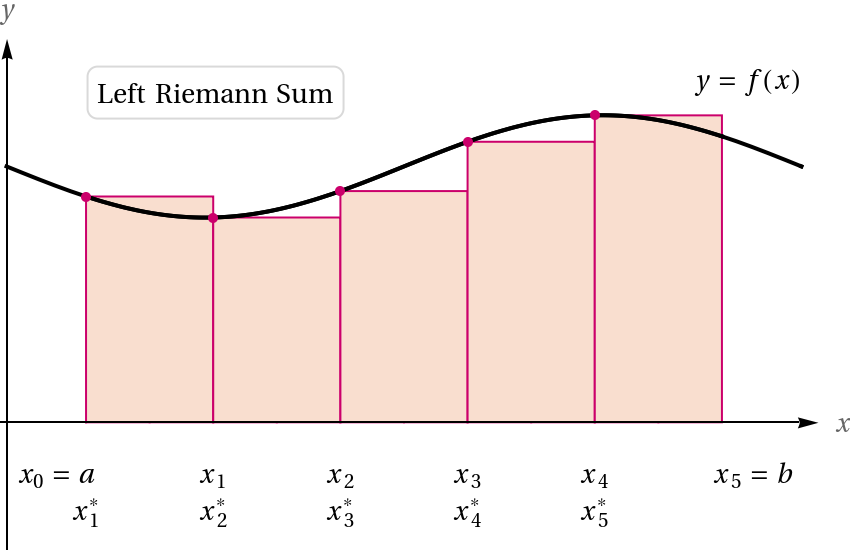
\includegraphics[width=\linewidth]{images/briggs_05_01/riemannSumLeft.png}&
      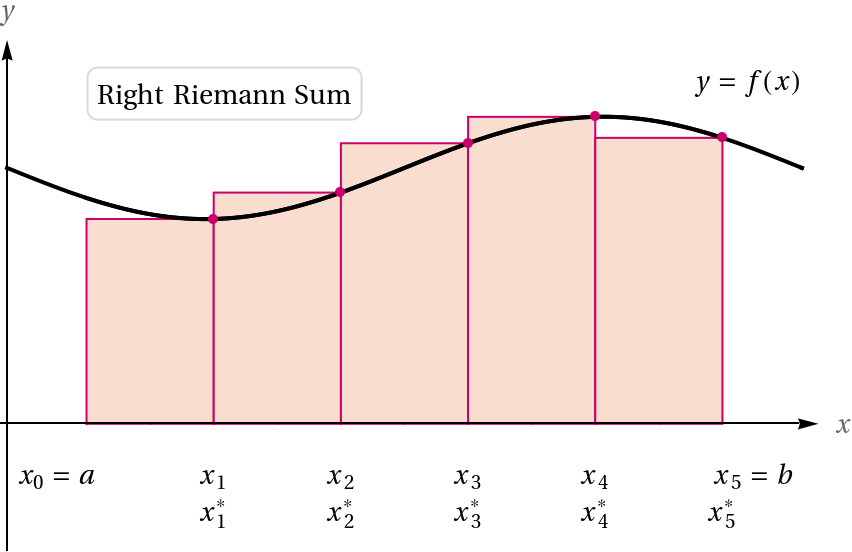
\includegraphics[width=\linewidth]{images/briggs_05_01/riemannSumRight.png}&
      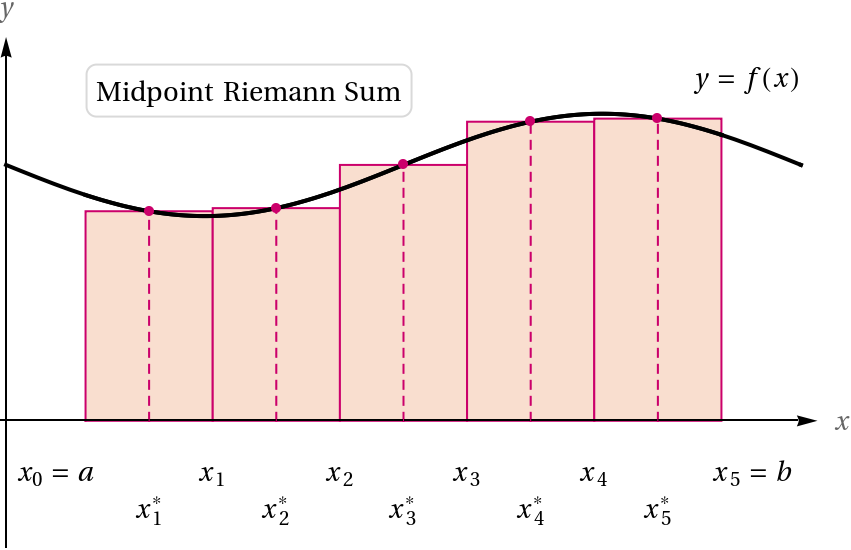
\includegraphics[width=\linewidth]{images/briggs_05_01/riemannSumMid.png}
    \end{tabularx}
  \end{center}
  \vspace*{\stretch{1}}
  \begin{quote}
    \noindent
    When estimating the area under the graph on the interval $\sbrkt{a,b}$, we define
      \[\Delta x=\dfrac{b-a}{n}\]
    to be the width of the rectangles. The height of the rectangles is given by $f(x_i)$, where the $x_i$'s are $\Delta x$ apart.
  \end{quote}
  \vspace*{\stretch{1}}
  \pagebreak
  
  \begin{ex*}
    Use the plots below to estimate the area under the given graph of $f(x)$:
  \end{ex*}
  \def\plotOne{
  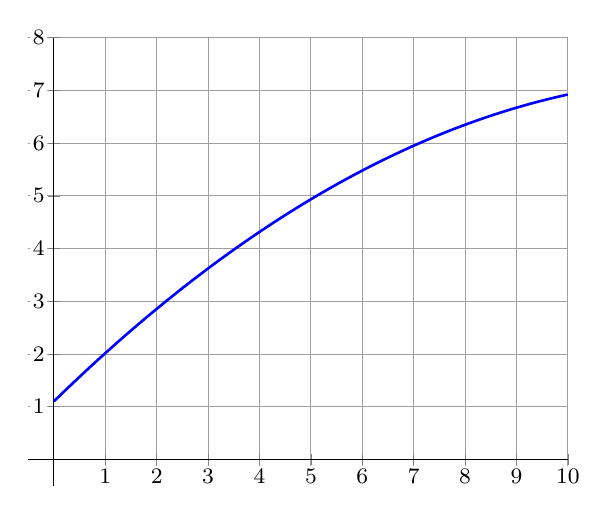
\begin{tikzpicture}
    \begin{axis}[
      grid=both,
      grid style={line width=0.35pt, draw=gray!75},
      axis lines=center,
      axis line style={-},
      xmin=-0.5, xmax=10,
      ymin=-0.5, ymax=8,
      xtick={0,1,...,10},
      ytick={0,1,...,8},
      ticklabel style={font=\footnotesize,inner sep=1pt,fill=white,opacity=1.0, text opacity=1},
      every axis plot/.append style={line width=0.95pt, color=blue, samples=100}
      ]
      \addplot[-] expression[domain=0:10] {-0.0369*x^2+0.95074*x+1.10261};
    \end{axis}
  \end{tikzpicture}
   }
  \begin{tasks}[after-item-skip=\stretch{1}, label=\mbox{}](1)
    \task 
      Sketch five rectangles and use them to find a lower estimate for the area under the given graph of $f(x)$ from $x=0$ to $x=10$.
      
      \begin{center}
        \plotOne
      \end{center}
    
    \task 
      Sketch five rectangles and use them to find a upper estimate for the area under the given graph of $f(x)$ from $x=0$ to $x=10$.
            
      \begin{center}
        \plotOne
      \end{center}
    
  \end{tasks}
  \vspace*{\stretch{1}}
  \pagebreak
  \def\plotTwo{
  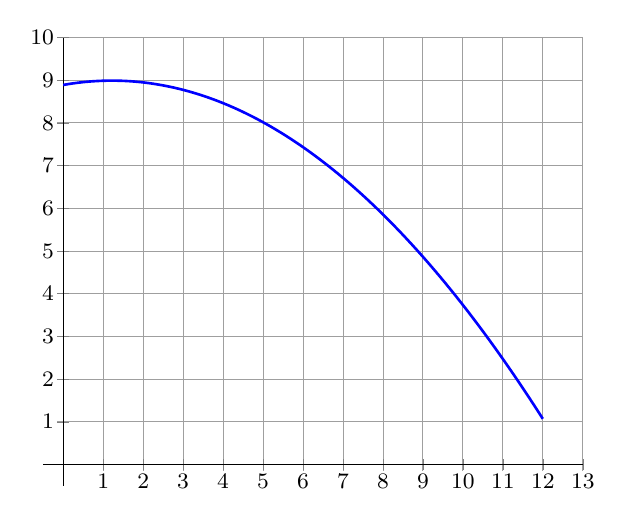
\begin{tikzpicture}
    \begin{axis}[
      grid=both,
      grid style={line width=0.35pt, draw=gray!75},
      axis lines=center,
      axis line style={-},
      xmin=-0.5, xmax=13,
      ymin=-0.5, ymax=10,
      xtick={0,1,...,13},
      ytick={0,1,...,10},
      ticklabel style={font=\footnotesize,inner sep=1pt,fill=white,opacity=1.0, text opacity=1},
      every axis plot/.append style={line width=0.95pt, color=blue, samples=100}
      ]
      \addplot[-] expression[domain=0:12] {-0.068154*x^2+0.16607*x+8.89047};
    \end{axis}
  \end{tikzpicture}
   }
  \begin{tasks}[after-item-skip=\stretch{1}, label=\mbox{}](1)
    \task 
      Use six right rectangles to estimate the area under the given graph of $f(x)$ from $x=0$ to $x=12$. Is the estimate an under-approximation or an over-approximation? Why?
      \begin{center}
        \plotTwo
      \end{center}
    
    \task 
      Use six midpoint rectangles to estimate the area under the given graph of $f(x)$ from $x=0$ to $x=12$. Talk about the quality of this estimate.
      \begin{center}
        \plotTwo
      \end{center}
  \end{tasks}
  \vspace*{\stretch{1}}
  \pagebreak
  
  \begin{ex*}
    Consider $f(x)=x^2$ on the interval $\sbrkt{0,1}$.
  \end{ex*}
  \newcommand{\blankAxis}{
    \begin{tikzpicture}[scale=0.775]
      \begin{axis}[
        axis lines=center,
        axis line style={-, line width=0.8pt},
        xmin=-0.125, xmax=1.25,
        ymin=-0.25, ymax=2,
        xtick={0.5,1},
        xticklabels={$\sfrac{1}{2}$,$1$},
        ymajorticks=false,
        minor x tick num=1,
        ticklabel style={font=\normalsize,inner sep=0.5pt,fill=white,opacity=1.0, text opacity=1},
        every axis plot/.append style={line width=0.95pt, color=blue, samples=100}
        ]
      \end{axis}
    \end{tikzpicture}
  }
  \begin{tasks}[after-item-skip=\stretch{1}](1)
    \task 
      Use two rectangles of equal width to find a lower sum for the area under the graph of $f(x)$.
      
      \blankAxis
    \task 
      Use four rectangles of equal width to find an upper sum for the area under the graph of $f(x)$.
      
      
      \blankAxis
    \task 
      Use four midpoint rectangles of equal width to estimate the area under the graph of $f(x)$.
      
      \blankAxis
  \end{tasks}
  \vspace*{\stretch{1}}
  \pagebreak
  
  \renewcommand{\blankAxis}{
    \begin{tikzpicture}[scale=0.775]
      \begin{axis}[
        axis lines=center,
        axis line style={-, line width=0.8pt},
        xmin=-0.525, xmax=5.25,
        ymin=-0.25, ymax=2,
        xtick={1,2,...,5},
        xticklabels={,$2$,,$4$,},
        ymajorticks=false,
        minor x tick num=0,
        ticklabel style={font=\normalsize,inner sep=0.5pt,fill=white,opacity=1.0, text opacity=1},
        every axis plot/.append style={line width=0.95pt, color=blue, samples=100}
        ]
      \end{axis}
    \end{tikzpicture}
  }
  \begin{ex*}
    Consider $f(x)=\dfrac{1}{x}$ on the interval $\sbrkt{1,5}$.
  \end{ex*}

  \vspace*{-10pt}

  \begin{tasks}[after-item-skip=\stretch{1}](1)
    \task 
      Use two rectangles of equal width to find a lower sum for the area under the graph of $f(x)$.
      
      \blankAxis
    \task 
      Use four rectangles of equal width to find a lower sum for the area under the graph of $f(x)$.
      
      \blankAxis
    \task 
      Use two rectangles of equal width to find an upper sum for the area under the graph of $f(x)$.
      
      \blankAxis
  \end{tasks}
  \vspace*{\stretch{1}}
  \pagebreak
  
  \begin{tasks}[after-item-skip=\stretch{1}, resume](1)
    \task 
      Use four rectangles of equal width to find an upper sum for the area under the graph of $f(x)$.
      
      \blankAxis
    \task 
      Use two midpoint rectangles of equal width to estimate the area under the graph of $f(x)$.
      
      \blankAxis
    \task 
      Use four midpoint rectangles of equal width to estimate the area under the graph of $f(x)$.
      
      \begin{tikzpicture}[scale=0.775]
        \begin{axis}[
          axis lines=center,
          axis line style={-, line width=0.8pt},
          xmin=-0.525, xmax=5.25,
          ymin=-0.25, ymax=2,
          xtick={1,2,...,5},
          xticklabels={,$2$,,$4$,},
          ymajorticks=false,
          minor x tick num=1,
          ticklabel style={font=\normalsize,inner sep=0.5pt,fill=white,opacity=1.0, text opacity=1},
          every axis plot/.append style={line width=0.95pt, color=blue, samples=100}
          ]
        \end{axis}
      \end{tikzpicture}
  \end{tasks}
  \vspace*{\stretch{1}}
  \pagebreak
  
  \begin{ex*}
    Use the tabulated values of $f$ to evaluate both the left and right Riemann sums. ($n=8$, $\sbrkt{1,5}$)
  \end{ex*}
  \begin{center}
    \begin{tabular}{@{}L*{9}{|>{\raggedleft\arraybackslash}p{0.35in}}@{}}
      x& 1& 1.5& 2& 2.5& 3& 3.5& 4& 4.5& 5\\\hline
      f(x)& 0& 2& 3& 2& 2& 1& 0& 2& 3
    \end{tabular}
  \end{center}
  \vspace*{\stretch{1}}
  
  \noindent
  When velocity is a continuous function, the area between the curve and the $x$-axis gives the displacement.
  \begin{ex*}
    The velocities (in $m/s$) of an automobile moving along a straight freeway over a four-second period are given in the following table. Find the midpoint Riemann sum approximation to the displacement on $\sbrkt{0,4}$ with $n=2$ and $n=4$ subintervals.
  \end{ex*}
  \begin{center}
    \begin{tabular}{@{}L*{9}{|>{\raggedleft\arraybackslash}p{0.35in}}@{}}
      t   &  0& 0.5&  1& 1.5&  2& 2.5&  3& 3.5& 4\\\hline
      v(t)& 20&  25& 30&  35& 30&  30& 35&  40& 40
    \end{tabular}
  \end{center}
  \vspace*{\stretch{1}}
  \pagebreak
  
  \begin{ex*}
    Use the following table of recorded velocities answer the following questions:
  \end{ex*}
  \begin{center}
    \begin{tabular}{@{}*{2}{p{0.775in}}|*{2}{>{\raggedleft\arraybackslash}p{0.775in}}@{}}\hline
      \lnret[l]{\textbf{Time}\\\textbf{(min)}}& 
      \lnret[l]{\textbf{Velocity}\\\textbf{(m/sec)}}& 
      \lnret[l]{\textbf{Time}\\\textbf{(min)}}& 
      \lnret[l]{\textbf{Velocity}\\\textbf{(m/sec)}}\\\hline
      %
       0& 1.0& 35& 1.2\\
       5& 1.2& 40& 1.0\\
      10& 1.7& 45& 1.8\\
      15& 2.0& 50& 1.5\\
      20& 1.8& 55& 1.2\\
      25& 1.6& 60& 0\\
      30& 1.4&\\\hline
    \end{tabular}
  \end{center}
  \begin{tasks}[after-item-skip=\stretch{1}](1)
    \task 
      Estimate the total displacement using 12 subintervals of length 5 with left-endpoint values.
    \task 
      Estimate the total displacement using 12 subintervals of length 5 with right-endpoint values.
  \end{tasks}
  \vspace*{\stretch{1}}
  \pagebreak
  
  \begin{defn*}
    If $a_m, a_{m+1},\dots,a_n$ are real numbers and $m$ and $n$ are integers such that $m\leq n$, then
      \[\sum\ito[m]^n a_i=a_m+a_{m+1}+\cdots+a_\nmo+a_n\]
  \end{defn*}
  \begin{ex*}
    Rewrite the sums without sigma notation and evaluate:
  \end{ex*}
  \begin{tasks}(2)
    \task $\ds\sum\kto^3 \frac{k-1}{k}$
    \task $\ds\sum\kto^4 \parens{-1}^k \cos(k\pi)$
  \end{tasks}
  \vspace*{\stretch{1}}
  \begin{ex*}
    Rewrite the following sum without sigma notation. Note that $n$ denotes the number of rectangles and the letters $i$, $j$, and $k$ are typically used for indexing.
      \[\sum\kto^n \frac{1}{n}(k^2+1)\]
  \end{ex*}
  \vspace*{\stretch{1}}
  \pagebreak
  
  \begin{ex*}
    Which of the following summations represent the sum $1+2+4+8+16+32$?
    \begin{tasks}(3)
      \task $\ds\sum\kto^6 2^{k-1}$
      \task $\ds\sum\kto[0]^5 2^k$
      \task $\ds\sum\kto[-1]^4 2^{k+1}$
    \end{tasks}
  \end{ex*}
  \vspace*{\stretch{1}}
  
  \begin{ex*}
    Which of the following summations represent the sum $1-2+4-8+16-32$?
    \begin{tasks}(3)
      \task $\ds\sum\kto^6 (-2)^{k-1}$
      \task $\ds\sum\kto[0]^5 (-1)^k2^k$
      \task $\ds\sum\kto[-2]^3 (-1)^{k+1}2^{k+2}$
    \end{tasks}
  \end{ex*}
  \vspace*{\stretch{1}}
  \pagebreak
  
  \begin{ex*}
    Express the following sums in sigma notation:
  \end{ex*}
  \begin{tasks}[after-item-skip=\stretch{1}](2)
    \task $-1+4-9+16-25$
    \task $\dfrac{1}{2}+\dfrac{1}{4}+\dfrac{1}{8}+\dfrac{1}{16}$
    \task $\dfrac{5}{2}+\dfrac{10}{3}+\dfrac{15}{4}+\dfrac{20}{5}+\dfrac{25}{6}+\dfrac{30}{7}$
    \task $4+9+14+\cdots+44$
  \end{tasks}
  \vspace*{\stretch{1}}
  
  \begin{ex*}
    Suppose that $\Sum\kto^n a_k=0$ and $\Sum\kto^n b_k=1$, evaluate the following
  \end{ex*}
  \begin{tasks}[after-item-skip=\stretch{1}](2)
    \task $\ds\sum\kto^n 8a_k$
    \task $\ds\sum\kto^n 250b_k$
    \task $\ds\sum\kto^n (a_k+1)$
    \task $\ds\sum\kto^n (b_k-1)$
  \end{tasks}
  \vspace*{\stretch{1}}
  \pagebreak
  
  \noindent
  \fbox{\parbox{0.9875\linewidth}{
    \textbf{Theorem 5.1: Sums of Powers of Integers}
    
    Let $n$ be a positive integer and $c$ a real number.
    \begin{align*}
      \sum\kto^n c&=cn& 
      \sum\kto^n k &=\frac{n(n+1)}{2}\\
      \sum\kto^n k^2&=\frac{n(n+1)(2n+1)}{6}&
      \sum\kto^n k^3&=\frac{n^2(n+1)^2}{4}
    \end{align*}
  }}
  
  \begin{ex*}
    Prove that $\ds\sum\kto^n k=\frac{n(n+1)}{2}$
  \end{ex*}
  \vspace*{\stretch{1}}
  \begin{ex*}
    Evaluate the following sums
  \end{ex*}
  \begin{tasks}[after-item-skip=\stretch{0.5}](3)
    \task $\ds\sum\kto^{10} k$
    \task $\ds\sum\kto^{10} \parens{1+k^2}$
    \task $\ds\sum\kto^{10} k^3$
    \task $\ds\sum\kto^7 (-2k-4)$
    \task $\ds\sum\kto^6 (3-k^2)$
    \task $\ds\sum_{m=1}^3 \frac{2m+2}{3}$
  \end{tasks}
  \vspace*{\stretch{0.5}}
  \pagebreak
  
  \begin{defn*}[Left, Right and Midpoint Riemann Sums in Sigma Notation]
    Suppose $f$ is defined on a closed interval $\sbrkt{a,b}$, which is divided into $n$ subintervals of equal length $\Delta x$. If $x_k^*$ is a point in the $k$th subinterval $\sbrkt{x_{k-1},x_k}$, for $k=1,2,\dots, n$, then the \textbf{Riemann sum} for $f$ on $\sbrkt{a,b}$ is $\ds\sum\kto^n f\parens{x_k^*}\Delta x$. Three cases arise in practice.
    \begin{itemize}
      \item 
        $\ds\sum\kto^n f(x_k^*)\Delta x$ is a \textbf{left Riemann sum} if $x_k^*=a+(k-1)\Delta x$.
      \item 
        $\ds\sum\kto^n f(x_k^*)\Delta x$ is a \textbf{right Riemann sum} if $x_k^*=a+k\Delta x$.
      \item 
        $\ds\sum\kto^n f(x_k^*)\Delta x$ is a \textbf{midpoint Riemann sum} if $x_k^*=a+(k-\sfrac{1}{2})\Delta x$.
    \end{itemize}
  \end{defn*}
  \begin{ex*}
    For the function $f(x)=3x^2$, find a formula for the upper sum obtained by dividing the interval $\sbrkt{0,1}$ into $n$ equal subintervals.
  \end{ex*}
  \vspace*{\stretch{1}}
  \noindent
  Now take the limit of the sum as $n\to\infty$ to calculate the area under $f(x)=3x^2$ over $\sbrkt{0,1}$.
  \vspace*{\stretch{0.5}}
  \pagebreak
  
  \begin{ex*}
    For the function $f(x)=2x$, find a formula for the upper sum obtained by dividing the interval $\sbrkt{0,3}$ into $n$ equal subintervals.
  \end{ex*}
  \vspace*{\stretch{1}}
  \noindent
  Now take the limit of the sum as $n\to\infty$ to calculate the area under $f(x)=2x$ over $\sbrkt{0,3}$.
  \vspace*{\stretch{1}}
  \pagebreak
  
\end{document}
